\lstinputlisting[language=bash,basicstyle=\small]{python_codes/fieldstone_45/keywords}

\begin{center}
Code at \url{https://github.com/cedrict/fieldstone/tree/master/python_codes/fieldstone_45}
\end{center}

\par\noindent\rule{\textwidth}{0.4pt}

%%%%%%%%%%%%%%%%%%%%%%%%%%%%%%%%%%%%%%%%%%%%%%%%%%%%%%%%%%%%%%%%%%%%%%%%%%%%%%%%%%%%%%%%%%%%%%%%%%%%

The domain is a unit square. Only the pure advection equation is solved. The setup 
is identical to stone 43. $P_1$ triangular elements are used. Crank-Nicolson scheme is used.
 

\begin{center}
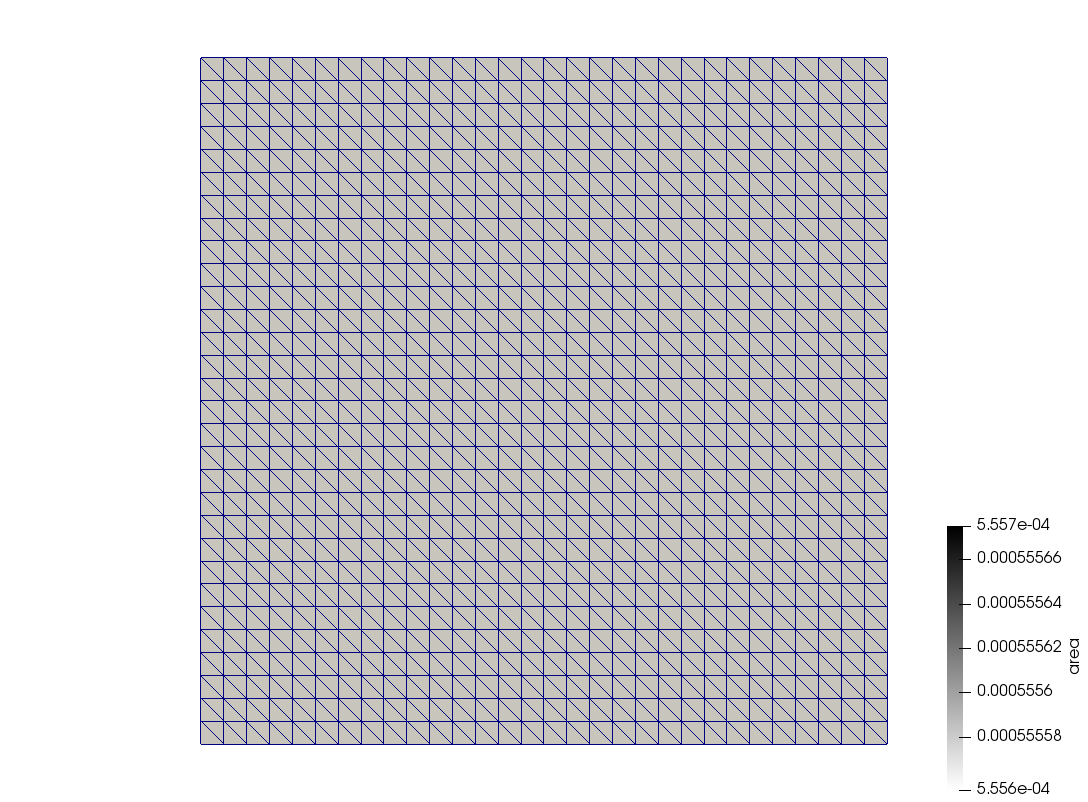
\includegraphics[width=8.5cm]{python_codes/fieldstone_45/results/mesh_reg}
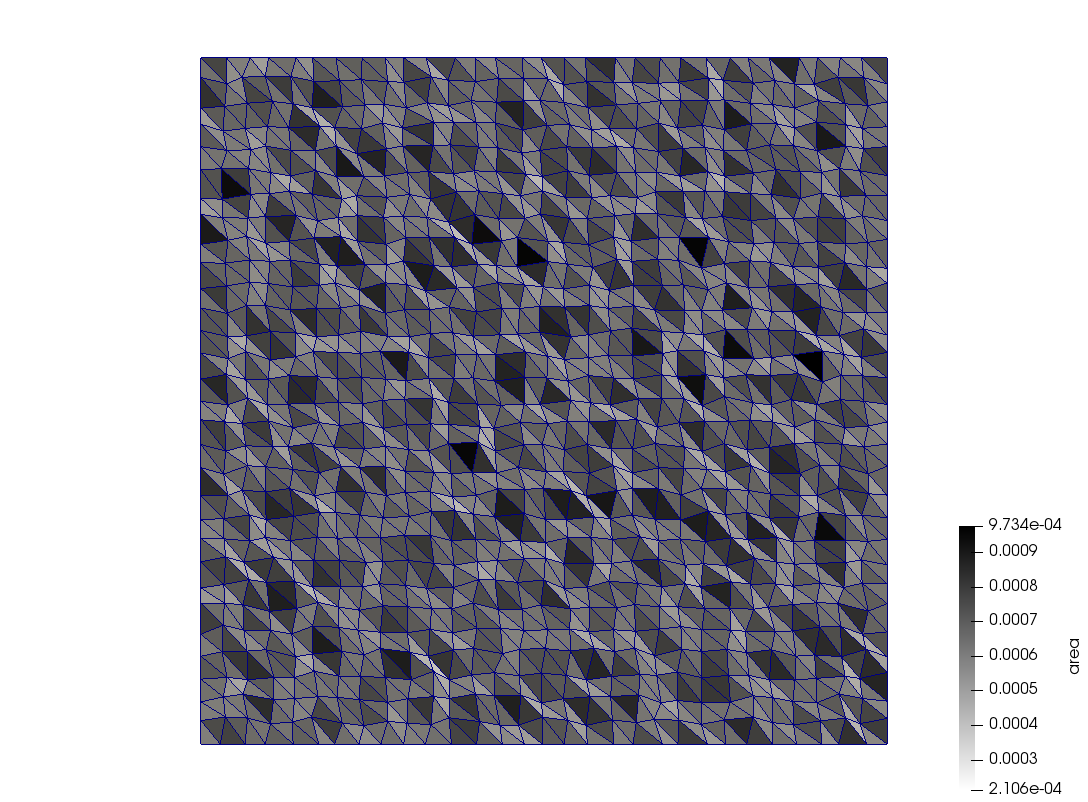
\includegraphics[width=8.5cm]{python_codes/fieldstone_45/results/mesh_rand}\\
{\captionfont Left: regular mesh of 30x30 cells; Right: same, with random noise added}
\end{center}

\begin{center}
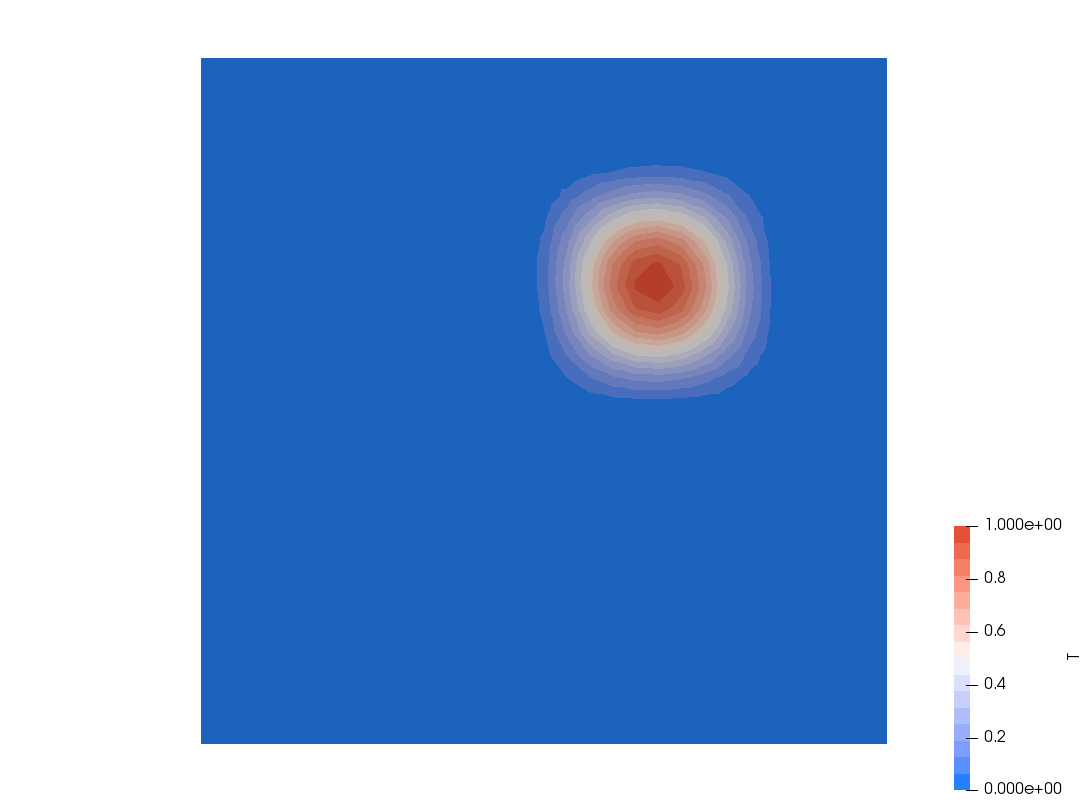
\includegraphics[width=5.6cm]{python_codes/fieldstone_45/results/reg0000}
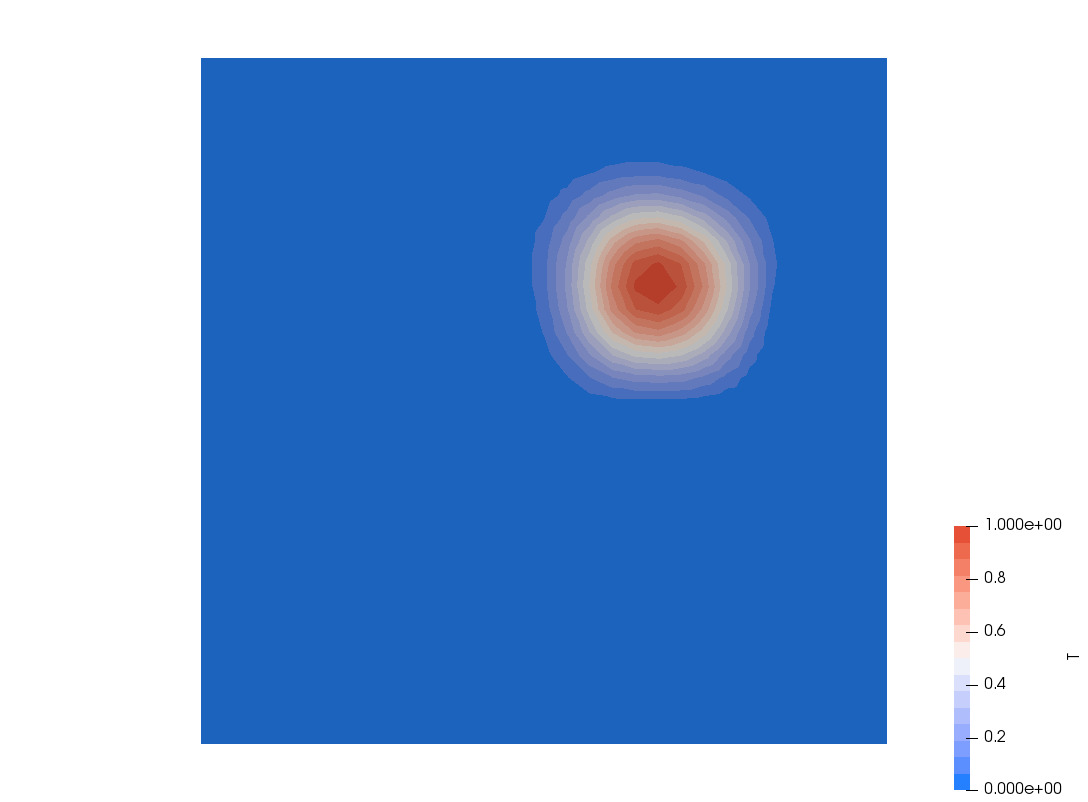
\includegraphics[width=5.6cm]{python_codes/fieldstone_45/results/reg0001}
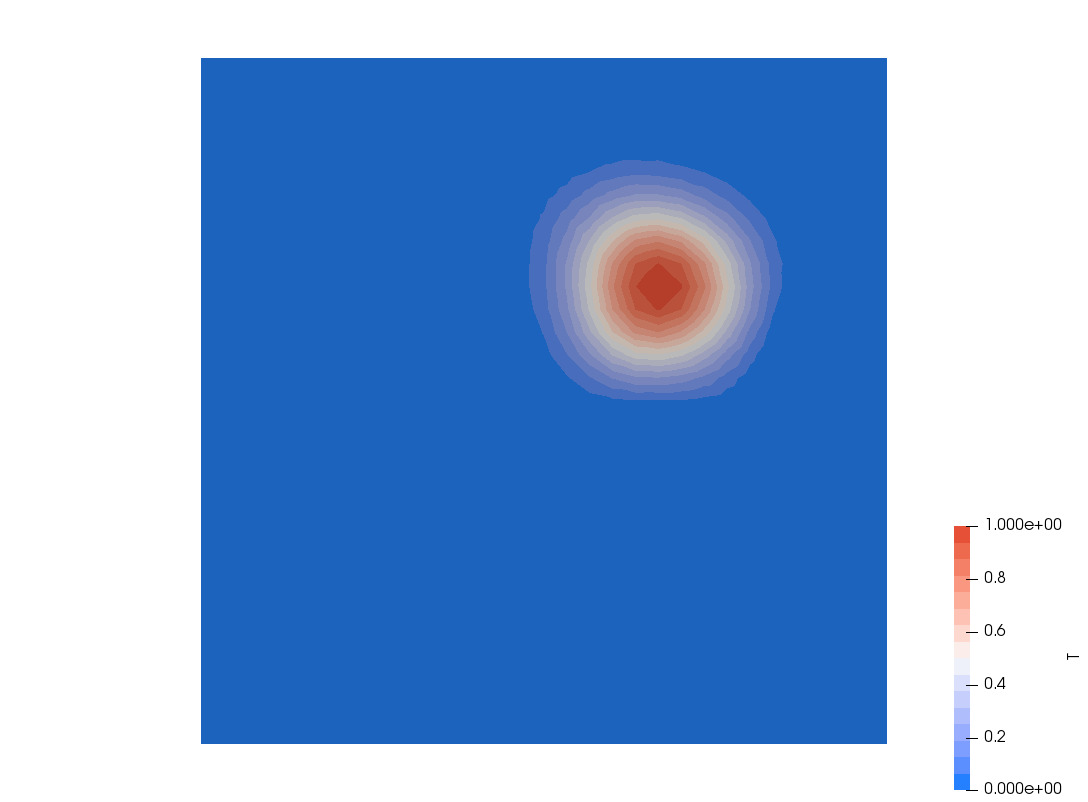
\includegraphics[width=5.6cm]{python_codes/fieldstone_45/results/reg0002}\\
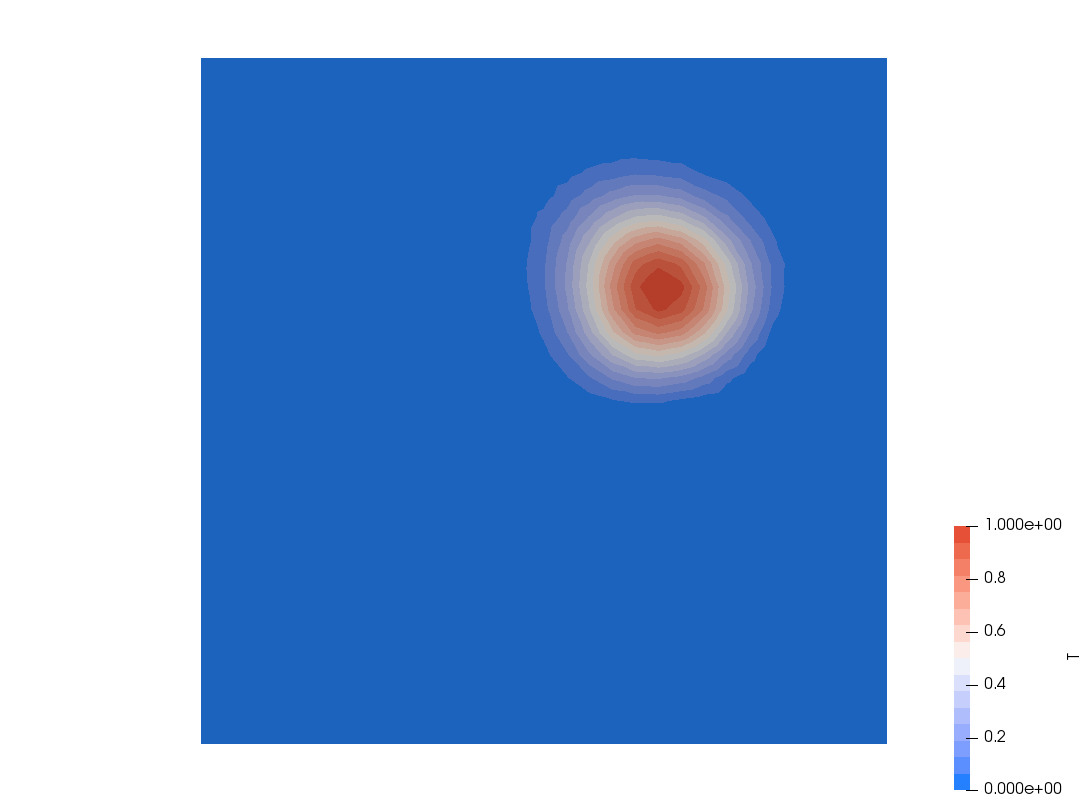
\includegraphics[width=5.6cm]{python_codes/fieldstone_45/results/reg0003}
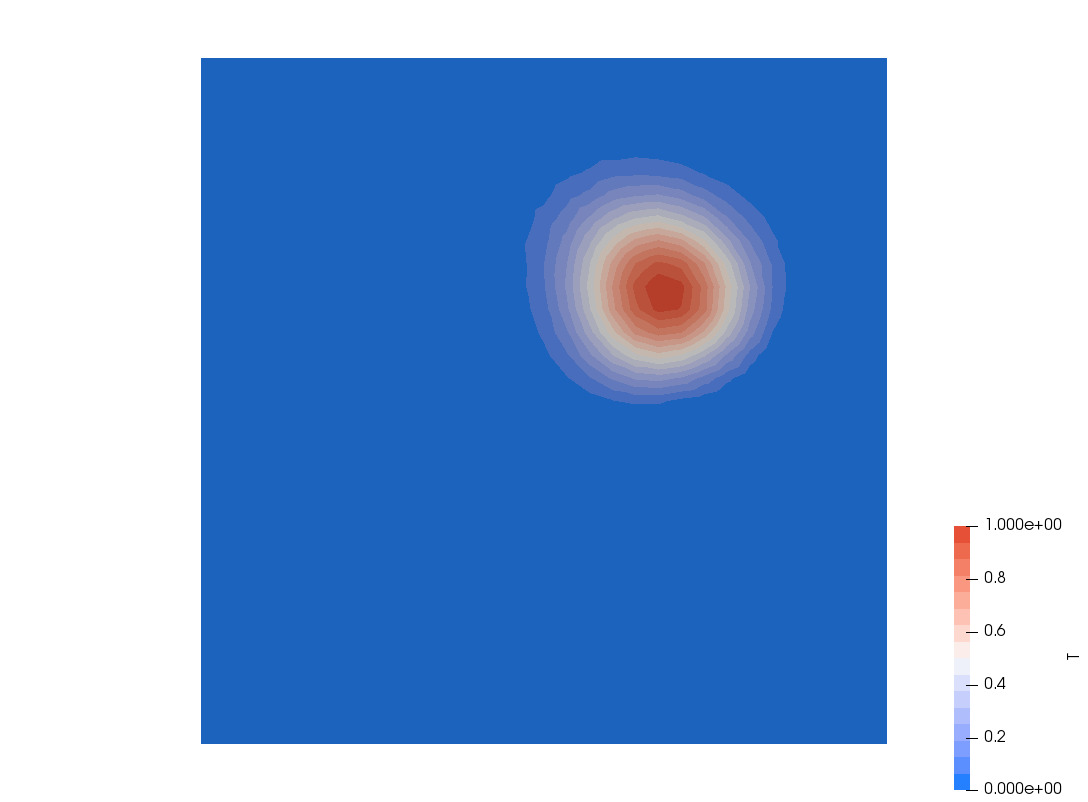
\includegraphics[width=5.6cm]{python_codes/fieldstone_45/results/reg0004}
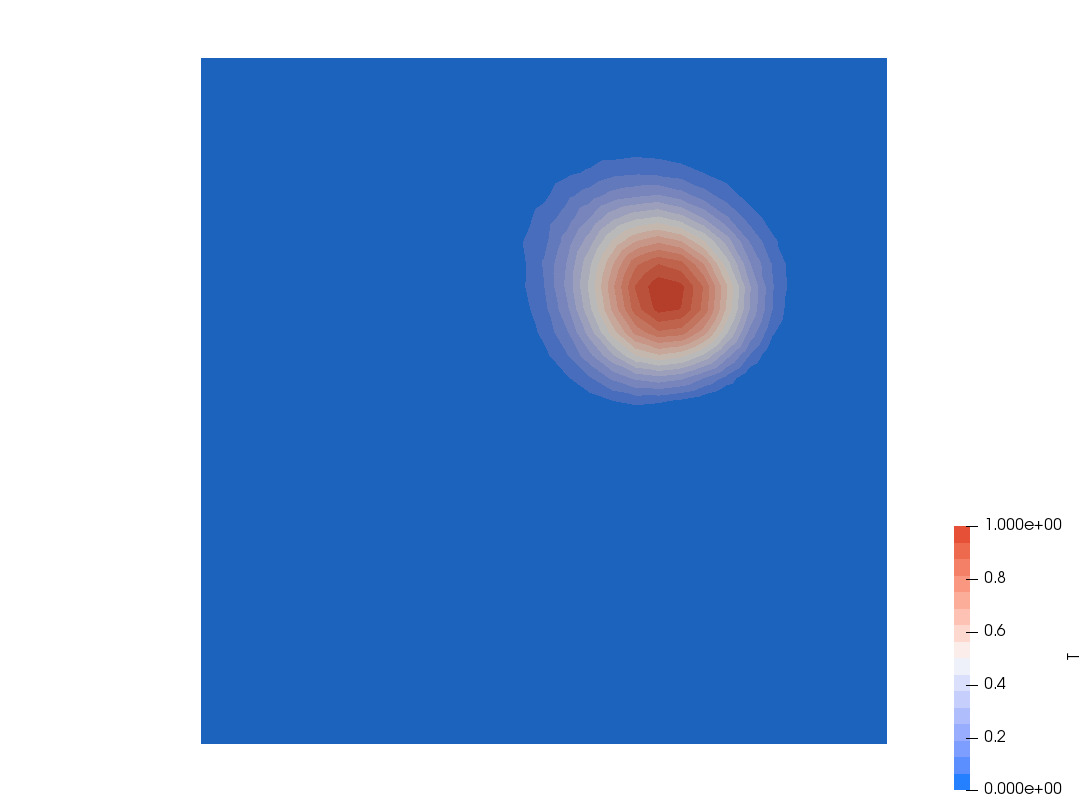
\includegraphics[width=5.6cm]{python_codes/fieldstone_45/results/reg0005}\\
{\captionfont Regular mesh. Temperature field after 0, $2\pi$, $4\pi$, $6\pi$, $8\pi$, $10\pi$ rotation}\\ 
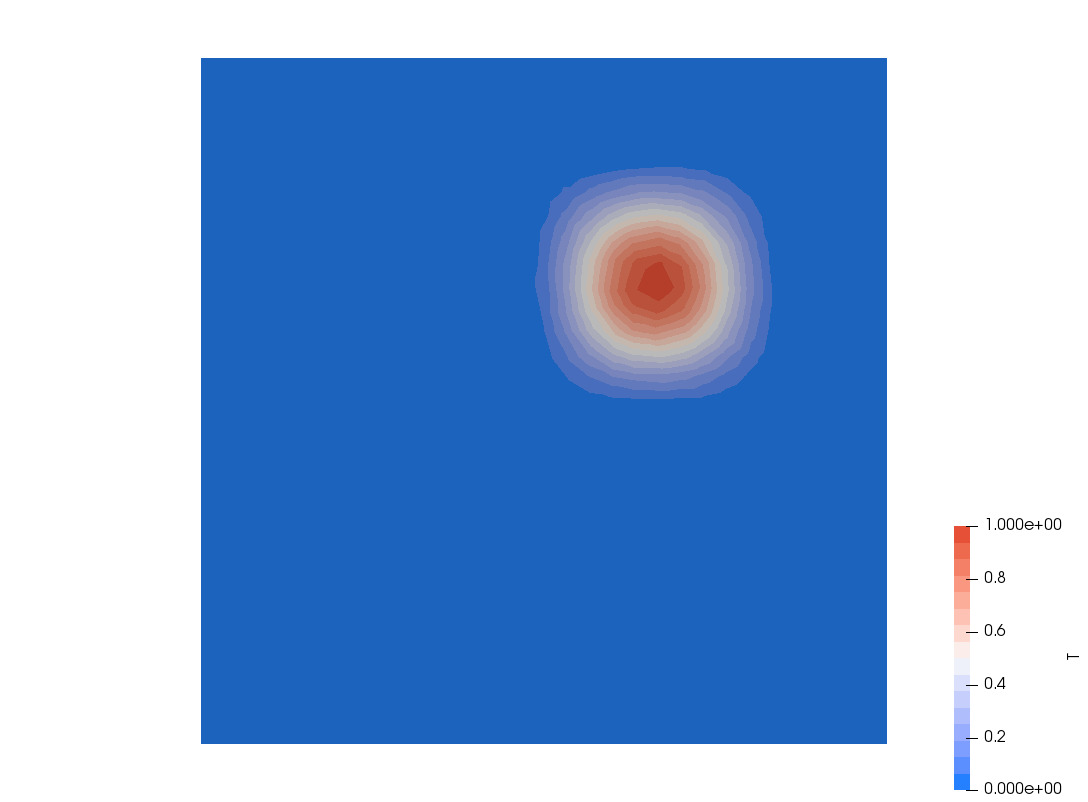
\includegraphics[width=5.6cm]{python_codes/fieldstone_45/results/rand0000}
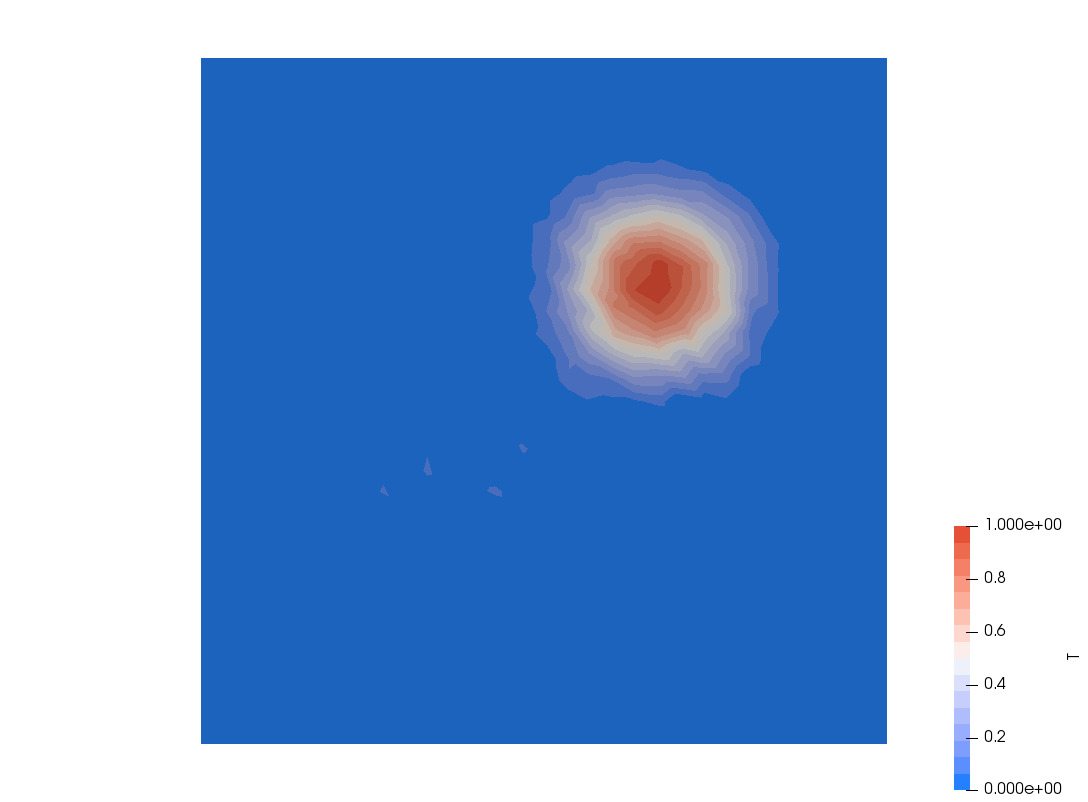
\includegraphics[width=5.6cm]{python_codes/fieldstone_45/results/rand0001}
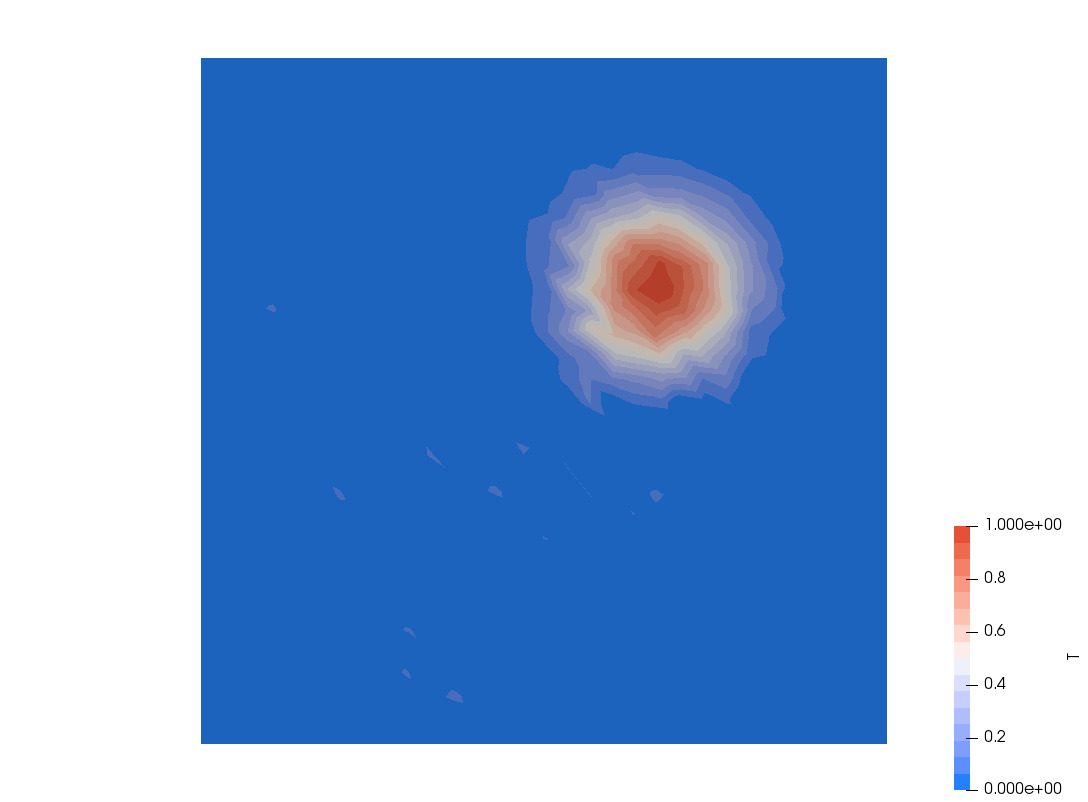
\includegraphics[width=5.6cm]{python_codes/fieldstone_45/results/rand0002}\\
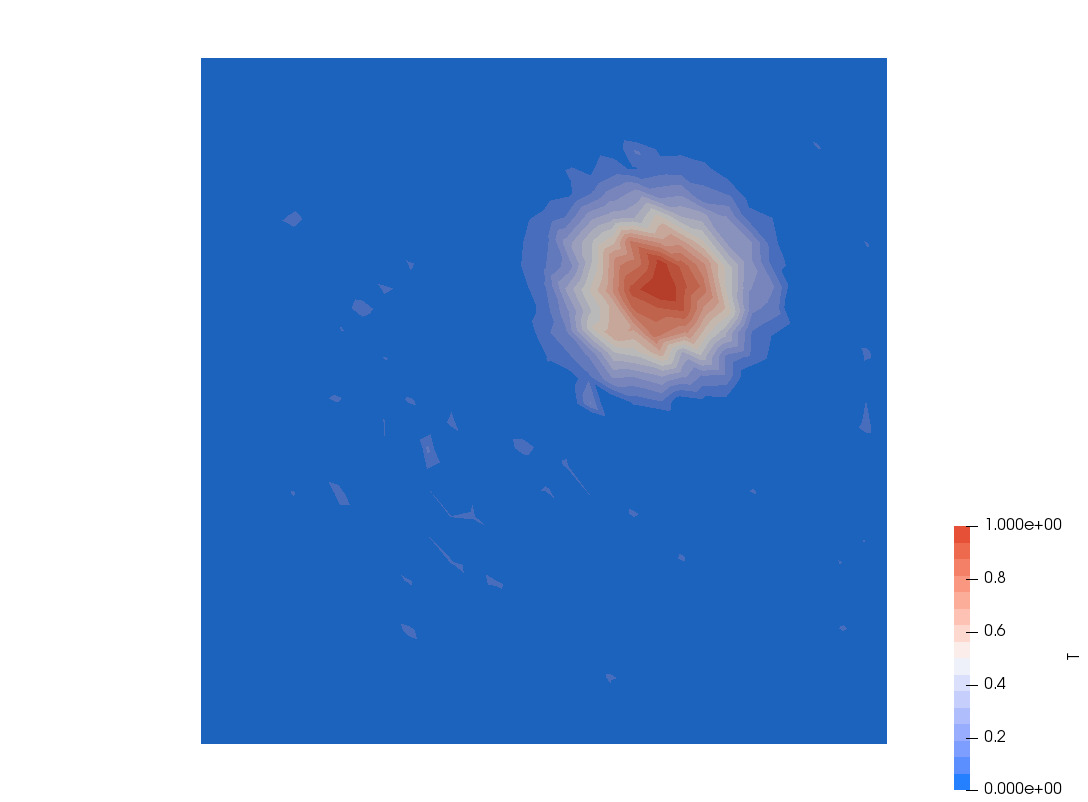
\includegraphics[width=5.6cm]{python_codes/fieldstone_45/results/rand0003}
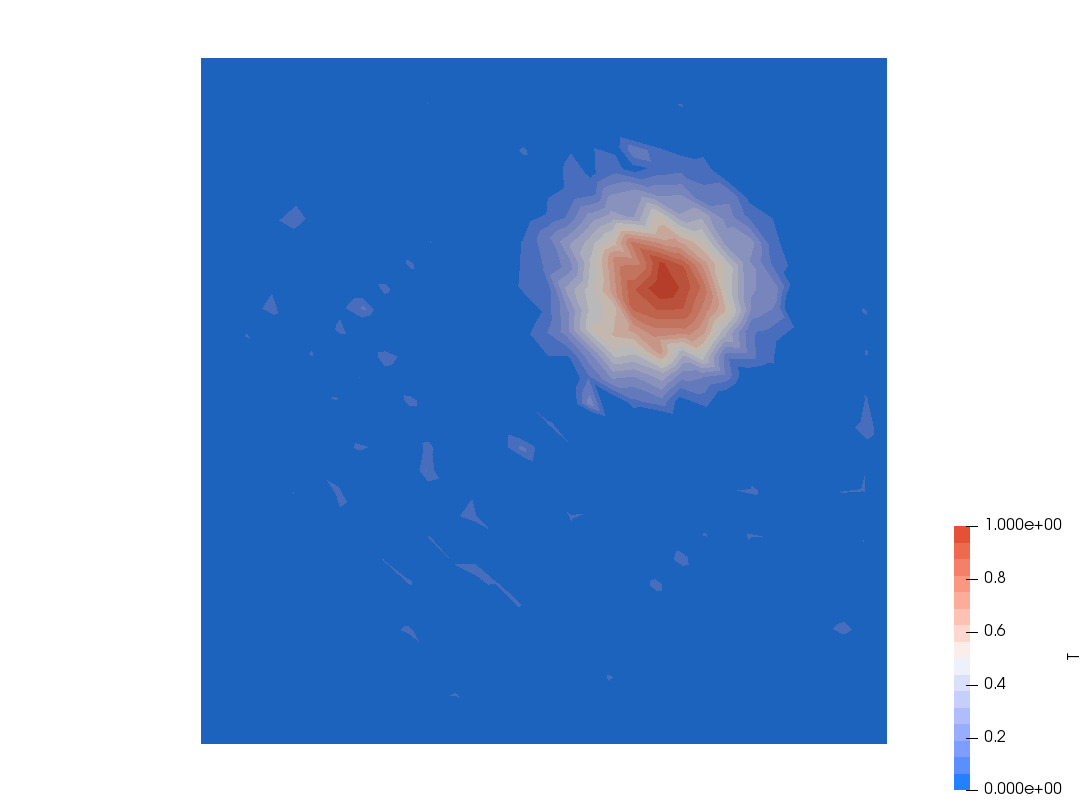
\includegraphics[width=5.6cm]{python_codes/fieldstone_45/results/rand0004}
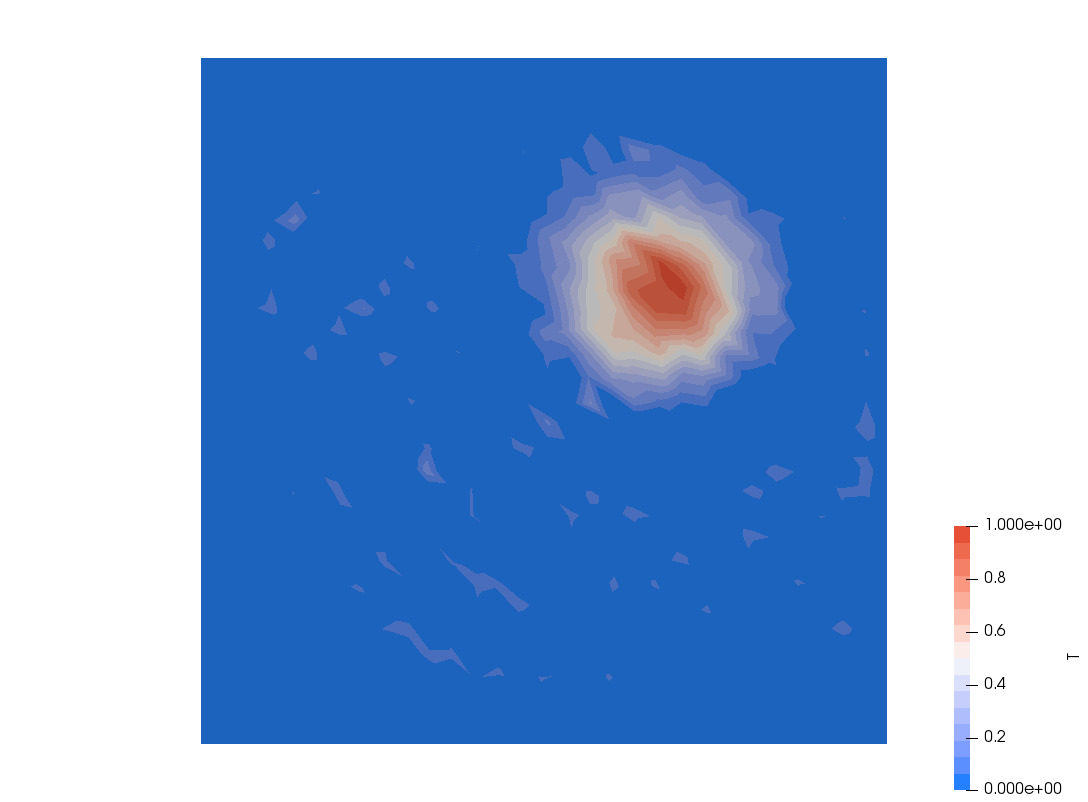
\includegraphics[width=5.6cm]{python_codes/fieldstone_45/results/rand0005}\\
{\captionfont Randomised mesh. Temperature field after 0, $2\pi$, $4\pi$, $6\pi$, $8\pi$, $10\pi$ rotation} 
\end{center}

\begin{center}
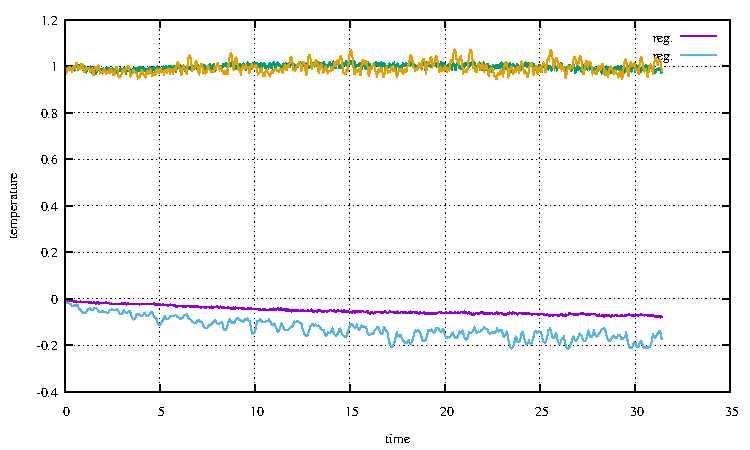
\includegraphics[width=10cm]{python_codes/fieldstone_45/results/T.pdf}\\
{\captionfont Minimum/maximum temperature as a function of time for both grids.} 
\end{center}
